\section{Entropy Regularization of Optimal Transport}
\label{sec:3}
\subsection{Background and Formulation}
\subsubsection{Kantorovich formulation of optimal transport}
\cite{COT} introduces the Kantorovich formulation of optimal transport (Kantorovich's relaxation). For two vectors $\mu\in\mbR^m$ and $\nu\in\mbR^n$, which satisfies $\mbone_n^T\mu=\mbone_m^T\nu$, we consider the following set of coupling matrices
\begin{equation}
U(\mu, \nu) \triangleq \left\{\pi\in\mbR^{m\times n}_+: \pi\mbone_n = \mu, \pi^T\mbone_m=\nu \right\}
\end{equation}
where we use the following matrix-vector notation
$$
\pi\mbone_n  = (\sum_j \pi_{i,j})_i\in\mbR^m, \quad \pi\mbone_m  = (\sum_i \pi_{i,j})_j\in\mbR^n,
$$

The Kantorovich's optimal transport problem reads
\begin{equation}
\label{equ:kot}
L_\mfc(\mu,\nu)\triangleq \min\limits_{\pi\in U(\mu, \nu)}\la C,\pi\ra\triangleq\sum_{i,j}C_{i,j}\pi_{i,j}
\end{equation}
Therefore, problem \ref{equ:kot} is equivalent to the standard form of LP \ref{lp}. 

\subsubsection{Entropy regularization}
For a coupling matrix $\pi \in U(\mu, \nu)$, the discrete entropy of $\pi$ is defined as
\begin{equation}
H(\pi)\triangleq-\sum_{i,j}\pi_{i,j}(\log(\pi_{i,j})-1)
\end{equation}
with an analogous definition for vectors, with the convention that $H(\pi) = -\infty$ if one of the entries $\pi_{i,j}$ is negative. Although discrete entropy is defined on matrices with positive entry, with $\lim\limits_{x\to0+}x(\log x-1)=0$, we can extend its definition to  matrices with non-negative entry. And we have
$$
H(\pi)=-\sum_{\pi_{i,j}\geqslant0}\pi_{i,j}(\log(\pi_{i,j})-1)
$$
Suppose $M=\min\{\|\mu\|_\infty, \|\nu\|_\infty\}$, then we have $\pi_{i,j}\leqslant\min\{\mu_i, \nu_j\}\leqslant M$. The function $H(\pi)$ is then $1/M$-strongly convex, because its Hessian is $\p^2H(\pi)=-\diag(1/\pi_{i,j})$. 

The idea of entropic regularization of optimal transport is to use $-H$ as a regularizing function to obtain approximate solutions to the Kantorovich's optimal transport problem \ref{equ:kot}. 

\begin{equation}
\label{equ:erot}
L^\epsilon_C(\mu,\nu)\triangleq \min\limits_{\pi\in U(\mu, \nu)}\la C,\pi\ra-\epsilon H(\pi)
\end{equation}

The convergence of the solution of that regularized problem towards an optimal solution of the original linear program has been studied by \cite{aaote}. 
\begin{proposition}[Convergence with $\epsilon$]
\label{sh_cvg}
The unique solution $\pi^\epsilon$ of \ref{equ:erot} converges to the optimal solution with maximal entropy within the set of all optimal solutions of the Kantorovich problem, namely
\begin{equation}
\label{sh_limit}
\pi^\epsilon\to\arg\min\limits_\pi\{-H(\pi): \pi\in U(\mu,\nu), \la\pi, C\ra=L_C(\mu,\nu)\}, \quad \epsilon\to0
\end{equation}
so that in particular
$$
L^\epsilon_C(\mu,\nu)\to L_C(\mu,\nu), \quad \epsilon\to0
$$
\end{proposition}
\begin{proof}
We consider a sequence $\{\epsilon_l\}$ such that $\epsilon_l\to0$ and $\epsilon_l>0$. We denote $\pi^l$ the solution to \ref{equ:erot} for $\epsilon=\epsilon_l$. Since $U(\mu,\nu)$ is bounded, we can extract a sequence (that we do not relabel for sake of simplicity) such that $\pi^l\to\pi^*$. Since $U(\mu, \nu)$ is closed, $\pi^*\in U(\mu,\nu)$. We consider any $\pi$ such that $\la C,\pi\ra=L_C(\mu,\nu)$. By the optimality of $\pi$ and $\pi^l$ for their respective optimization problem, we have
\begin{equation}
0\leqslant\la C, \pi^l\ra-\la C, \pi\ra\leqslant\epsilon_l(H(\pi^l)-H(\pi))
\end{equation}
Since $H$ is continuous, taking the limit $l\to\infty$ in this expression shows that $\la C, \pi^*\ra=\la C, \pi\ra$ so that $\pi^*$ is a feasible point of \ref{sh_limit}. Furthermore, we have $H(P^*)\geqslant H(P)$, which shows that $P^*$ is the solution to \ref{sh_limit}. By strict convexity of $-H$, the solution is unique and the whole sequence is converging. 
\end{proof}

The following figures \ref{gmm1} and \ref{gmm2} illustrates the impact of $\epsilon$ on the coupling $\pi$ between two Gaussian mixture models.
\begin{figure}[!htb]
\centering
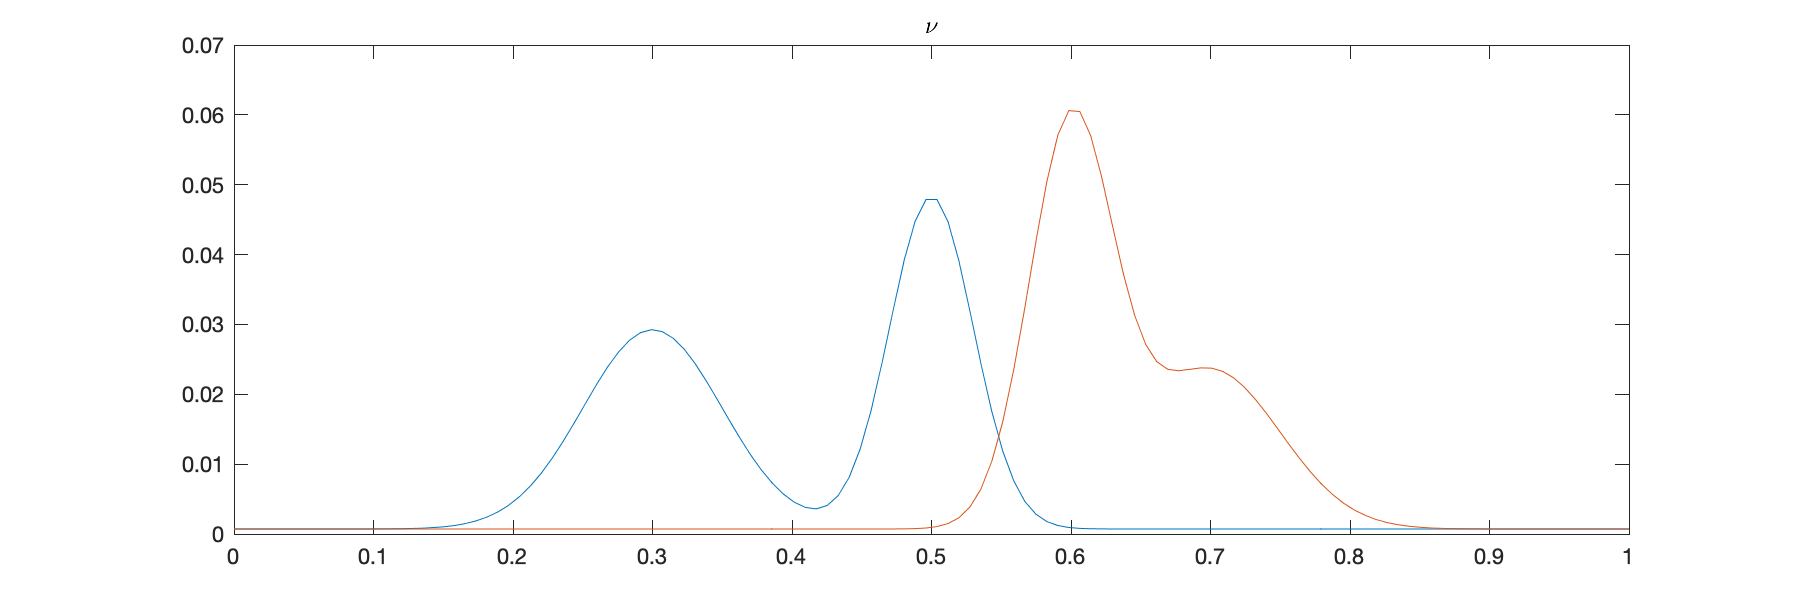
\includegraphics[width=12cm]{final/gmm1.png}
\caption{The probability distribution function of two Gaussian mixture models $G_1$ and $G_2$. $G_1$ (blue one) has mean $[0.3,0.5]$, variance $[0.05^2, 0.03^2]$ and component proportion $[0.5, 0.5]$; $G_2$ (red one) has mean $[0.6,0.7]$, variance $[0.03^2, 0.05^2]$ and component proportion $[0.6, 0.4]$. }
\label{gmm1}
\end{figure}

\begin{figure}[!htb]
\centering
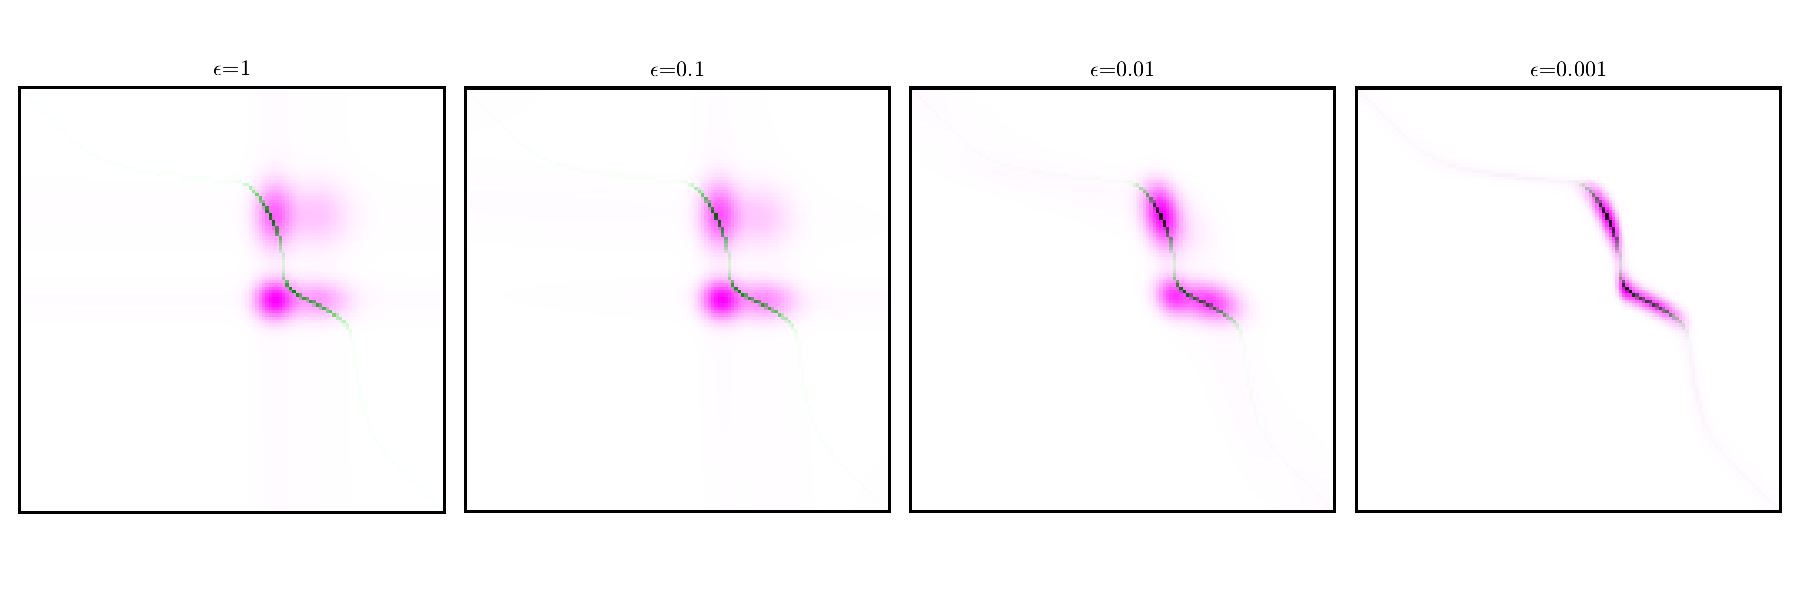
\includegraphics[width=12cm]{final/gmm2.png}
\caption{Impact of $\epsilon$ on the coupling between two gaussian mixture models \ref{gmm1}. From left to right, $\epsilon=1,0.1,0.01,0.001$. The purple one is the solution to the entropy regularized LP. The green one is the solution to the original LP.}
\label{gmm2}
\end{figure}

Define the Kullback-Leibler divergence between couplings as
$$
\mathrm{KL}(\pi|K)\triangleq\sum_{i,j}\pi_{i,j}\log(\frac{\pi_{i,j}}{K_{i,j}})-\pi_{i,j}+K_{i,j}
$$
We take $K^\epsilon_{i,j}\triangleq e^{-\frac{C_{i,j}}{\epsilon}}$, the Gibbs kernel associated to the cost matrix $C$. The unique solution $\pi^\epsilon$ of \ref{equ:erot} is a projection onto $U(\mu,\nu)$, namely
$$
\pi^\epsilon\triangleq\arg\min\limits_{\pi\in U(\mu,\nu)}\mathrm{KL}(\pi|K^\epsilon)
$$

\subsubsection{Formulation of the problem}
The optimization problem of the entropic regularization of optimal transport with parameter $\epsilon$ is given by:
\begin{equation}
\label{equ:kl}
\left\{
\begin{aligned}
&\min \, \la C,\pi\ra-\epsilon H(\pi)=\mathrm{KL}(\pi|K^\epsilon)\\
&\mathrm{s.t.}\, \pi\in U(\mu, \nu)
\end{aligned}\right.
\end{equation}
where $K^\epsilon_{i,j}= e^{-\frac{C_{i,j}}{\epsilon}}$.

\subsection{Sinkhorn's Algorithm}
We start with the following proposition. 

\begin{proposition}
\label{sh_basic}
The solution to \ref{equ:kl} is unique and has the form 
\begin{equation}
\label{equ:para}
\forall 1\leqslant i\leqslant m, 1\leqslant j\leqslant n, \quad \pi^\epsilon_{i,j}=a_iK^\epsilon_{i,j}b_j
\end{equation}
for two (unknown) scaling variable $(a,b)\in \mbR_+^m\times\mbR_+^n$.  
\end{proposition}

\begin{proof}
Introducing two dual variable $f\in\mbR^m, g\in\mbR^n$ for each marginal constraint. The Lagrangian of \ref{equ:kl} reads
$$
L(\pi,f,g)=\la\pi,C\ra-\epsilon H(P)-\la f, \pi\mbone_n-\mu\ra-\la g, \pi^T\mbone_m-\nu\ra
$$
The first order conditions yield
$$
\frac{\p L}{\p \pi_{i,j}}=C_{i,j}+\epsilon log(P_{i,j})-f_i-g_j=0
$$
This means that an optimal $\pi$ coupling to the regularized problem can be written as $P_{i,j}=e^{f_i/\epsilon}e^{-C_{i,j}/\epsilon}e^{g_j/\epsilon}$. Let $a=e^{f_i/\epsilon}, b= e^{g_j/\epsilon}$, then we have $$
\pi_{i,j}=a_iK^\epsilon_{i,j}b_j
$$
\end{proof}

This shows that the solution of \ref{equ:kl} has a specific form, which can be parameterized using $m+n$ variables.

The parameterization of the optimal solution in equation \ref{equ:para} can be written in the matrix form $\pi^\epsilon = \diag(a)K^\epsilon\diag(b)$. Then, $a,b$ must satisfies:
\begin{equation}
\diag(a)K^\epsilon\diag(b)\mbone_m=\mu, \quad \diag(a)K^T\diag(b)\mbone_n=\nu
\end{equation}
These two equations can be further simplified as
\begin{equation}
a\odot (K^\epsilon b)=\mu, \quad b\odot\left((K^\epsilon)^Ta\right)=\nu
\end{equation}
where $\odot$ corresponds to entry-wise multiplication of vectors. The Sinkhorn's algorithm iteratively update $a^{(l+1)}$ and $b^{(l+1)}$ by
\begin{equation}
\label{upd_sh}
a^{(l+1)}=\frac{\mu}{K^\epsilon b^{(l)}}, \quad b^{l+1}=\frac{\nu}{(K^\epsilon)^Ta^{(l+1)}}
\end{equation}
initialized with an arbitrary positive vector $b^{(0)}=\mbone_n$. The division operator used above between two vectors is to be understood entry-wise. The whole algorithm is given by:

\begin{algorithm}
\caption{Sinkhorn's algorithm}
\label{alg:sa}
\begin{algorithmic}[1]
\REQUIRE $\epsilon$, $C\in\mbR^{m\times n}$, $\mu\in\mbR^m$, $\nu\in\mbR^n$.
\STATE Start with $b^{(0)}=\mbone_n$, $l=0$
\STATE Calculate $K^\epsilon_{i,j}= e^{-\frac{C_{i,j}}{\epsilon}}$
\WHILE {\text{not converge}}
	\STATE Update $a^{(l+1)}$ and $b^{(l+1)}$ by \ref{upd_sh}, $l=l+1$
\ENDWHILE
\STATE $a=a^{(l)}, b=b^{(l)}$
\RETURN $\pi=\diag(a)K^\epsilon \diag(b)$
\end{algorithmic}
\end{algorithm}

This algorithm was originally introduced with a proof of convergence by \cite{sinkhorn}. For simplicity, we assume $m=n$. \cite{nltaa} showed that by setting $\epsilon=\frac{\tau}{4\log(n)}$, $O(\|C\|_\infty^3\log(n)\tau^{-3})$ Sinkhorn iterations (with an additional
rounding step to compute a valid coupling $\hat\pi\in U(\mu,\nu)$) are enough to ensure $\la \hat \pi, C\ra\leqslant L_C(\mu,\nu)+\tau$. This implies that Sinkhorn computes a $\tau$-approximate solution of the unregularized OT problem in $O(n^2\log(n)\tau^{-3})$ operations. The rounding scheme consists in, given two vectors $a\in\mbR^m, \, b\in\mbR^n$ to carry out the following updates:
$$
a'=a\odot \min\left(\frac{\mu}{a\odot(K^\epsilon b)},\mbone_m\right), \quad b'=b\odot \min \left(\frac{\nu}{b\odot((K^\epsilon)^Ta')},\mbone_n\right)
$$
$$
\Delta_\mu = \mu-a'\odot(K^\epsilon b'), \quad \Delta_\nu=\nu-b'\odot\left((K^\epsilon)^Ta'\right)
$$
$$
\hat \pi = \diag(a') K^\epsilon\diag (b')+\Delta_\mu\Delta_\nu^T/\|\Delta_\mu\|_1
$$
This yields a matrix $\hat\pi\in U(\mu,\nu)$ such that the $1$-norm of $\hat \pi -\diag(a) K^\epsilon\diag (b) $ is controlled by the marginal violations of $\diag(a)K^\epsilon\diag(b)$, namely
$$
\|\hat \pi -\diag(a) K^\epsilon\diag (b')\|_1\leqslant\|\mu-a\odot(K^\epsilon b)\|_1+\|\nu-b\odot\left((K^\epsilon)^Ta\right)\|_1
$$
In actual implementation, this step is crucial to decrease the violation of constraints. 

\subsection{Our proposed algorithm}
\subsubsection{Sinkhorn's algorithm with numerical stability and continuation strategy}
We denote $\|C\|_\infty=\max\limits_{i,j}|C_{i,j}|$. In actual implementation of Sinkhorn's algorithm \ref{alg:sa}, because we have $K^\epsilon_{i,j}=e^{-\frac{C_{i,j}}{\epsilon}}$, when $\epsilon$ is small, namely $\epsilon<\frac{\|C\|_\infty}{806}$, the largest entry of $K$ is smaller than $e^{-806}\approx 10^{-350}$. Most of the entry of $K^{\epsilon}$ would be rounded to $0$ because they are smaller than the smallest positive number that the computer can restore. If we want to calculate $K^\epsilon$, we would have a positive lower bound $\frac{\|C\|_\infty}{806}$ for $\epsilon$. This is not desired and it would make the result from proposition \ref{sh_cvg} meaningless.

We propose a numerical stable version of Sinkhorn's algorithm with no lower bound of $\epsilon$. A possible way to remove this lower bound of $\epsilon$ is to avoid directly calculating $K^\epsilon$ to update $a^{(l+1)}$ and $b^{(l+1)}$. Therefore, from the proof of proposition \ref{sh_basic}, we denote $a^{(l)}=e^{f^{(l)}/\epsilon}$, $b^{(l)}=e^{g^{(l)}/\epsilon}$, where $f^{(l)}\in R^m, g^{(l)}\in R^n$. Then, the update rule for $f^{(l+1)}$ and $g^{(l+1)}$ reads
\begin{equation}
\label{upd_sh_log}
f^{(l+1)}=\epsilon(\log(\mu)-\log(K^\epsilon e^{g^{(l)}/\epsilon})), \quad g^{(l+1)}=\epsilon(\log(\nu)-\log((K^\epsilon)^T e^{f^{(l+1)}/\epsilon})),
\end{equation}
Our motivation is to caculate $\log(K^\epsilon e^{g^{(l)}/\epsilon})$ and $\log((K^\epsilon)^T e^{f^{(l+1)}/\epsilon})$ in update rule \ref{upd_sh_log} in a numerically stable way. We start with the update of $f^{(l+1)}$. It is easy to verify that
$$
f^{(l+1)}_i = \epsilon \log(\mu_i)-\epsilon \log(\sum_{j=1}^ne^{(-C_{i,j}+g^{(l)}_j)/\epsilon})
$$
Directly calculating $\sum_{j=1}^ne^{(-C_{i,j}+g^{(l)}_j)/\epsilon}$ is dangerous because it might be rounded to $0$. Let $\hat f^{(l+1)}_i=\max_j\{-C_{i,j}+g^{(l)}_j\}$. Then, to update $f$ with numerical stability, we can update $f^{(l+1)}_i$ by
\begin{equation}
\label{sh_f_upd}
f^{(l+1)}_i = \epsilon \log(\mu_i)-\hat f^{(l)}_i-\epsilon \log(\sum_{j=1}^ne^{ (-C_{i,j}+g^{(l)}_j-\hat f^{(l)}_i)/\epsilon})
\end{equation}
Because $\sum_{j=1}^ne^{ (-C_{i,j}+g^{(l)}_j-\hat f^{(l)}_i)/\epsilon}\geqslant1$, to update $f^{(l+1)}$ in this way is safe. Actually, we use $\hat f_i^{(l)}/\epsilon+\log(\sum_{j=1}^ne^{ (-C_{i,j}+g^{(l)}_j-\hat f^{(l)}_i)/\epsilon})$ to calculate $\log(K^\epsilon e^{g^{(l)}/\epsilon})$.  Similarly, we let $\hat g^{(l+1)}_j=\max_i\{-C_{i,j}+f^{(l+1)}_i\}$, and update $g^{(l+1)}_j$ by
\begin{equation}
\label{sh_g_upd}
g^{(l+1)}_j = \epsilon \log(\nu_j)-\hat g^{(l+1)}_j-\epsilon \log(\sum_{i=1}^ne^{ (-C_{i,j}+f^{(l+1)}_i-\hat g^{(l+1)}_j)/\epsilon})
\end{equation}
In the end of the algorithm, we also use an additional rounding step to compute a valid coupling $\hat\pi$. Given two vectors $f\in\mbR^m, g\in\mbR^n$ and coupling matrix $\pi\in\mbR^{m\times n}$ with $\pi_{i,j}=e^{(f_i-C_{i,j}+g_j)/\epsilon}$, we compute $\hat\pi$ in the following way:
\begin{equation}
\label{add_coup}
\begin{aligned}
&\hat f_i=\max_j\{-C_{i,j}+g_j\}, \quad f'_i=f_i+\min\{\epsilon(\log(\mu_i)-\sum_{j=1}^ne^{ (-C_{i,j}+g_j-\hat f_i)/\epsilon})-\hat f_i-f_i,0\}\\
&\hat g_j=\max_i\{-C_{i,j}+f'_i\}, \quad g'_j=g_j+\min\{\epsilon(\log(\nu_j)-\sum_{i=1}^me^{ (-C_{i,j}+f'_i-\hat g_j)/\epsilon})-\hat g_j-g_j,0\}\\
&\hat f'_i=\max_j\{-C_{i,j}+g'_j\}, \quad (\Delta_\mu)_i=\mu_i-(\sum_{j=1}^ne^{ (-C_{i,j}+g'_j-\hat f'_i)/\epsilon})e^{(f'_i+\hat f'_i)/\epsilon}\\
&(\Delta_\nu)_j=\nu_j-(\sum_{i=1}^ne^{ (-C_{i,j}+f'_i-\hat g'_j)/\epsilon})e^{(g'_j+\hat g'_j)/\epsilon}, \quad \hat\pi=\pi+\Delta_\mu\Delta_\nu^T/\|\Delta_\mu\|_1
\end{aligned}
\end{equation}
Then, we get the following Sinkhorn's algorithm with numerical stability. It shares the same idea with Log-domain Sinkhorn's algorithm \cite{COT}. 
\begin{algorithm}
\caption{Sinkhorn's algorithm with numerical stability}
\label{alg:sans}
\begin{algorithmic}[1]
\REQUIRE $\epsilon$, $C\in\mbR^{m\times n}$, $\mu\in\mbR^m$, $\nu\in\mbR^n$.
\STATE Start with $g^{(0)}=\mathbf{0}_n$, $l=0$
\WHILE {\text{not converge}}
	\STATE Calculate $\hat f^{(l+1)}_i=\max_j\{-C_{i,j}+g^{(l)}_j\}$ and update $f^{(l+1)}$ by \ref{sh_f_upd}
	\STATE Calculate $\hat g^{(l+1)}_i=\max_i\{-C_{i,j}+f^{(l+1)}_i\}$ and update $g^{(l+1)}$ by \ref{sh_g_upd}, $l=l+1$
\ENDWHILE
\STATE Let $f=f^{(l)}, g=g^{(l)}$, calculate $\pi_{i,j}=e^{(f_i-C_{i,j}+g_j)/\epsilon}$, and compute $\hat\pi$ by \ref{add_coup}
\RETURN $\hat \pi$
\end{algorithmic}
\end{algorithm}

We shall point out that $\epsilon>0$ is vital in the iteration \ref{sh_f_upd} and \ref{sh_g_upd} because $f^{(l)}$ and $g^{(l)}$ will converge to the optimal solution to the dual problem of \ref{equ:kl} by Proposition \ref{sh_basic}. If we let $\epsilon\to 0$ in \ref{sh_f_upd} and \ref{sh_g_upd}, we would find that these updates become as follows:
\begin{equation}
\label{upd_div}
f_i^{(l+1)}=-\hat f_i^{(l)}=\min_j\{C_{i,j}-g^{(l)}_j\}, \quad g_j^{(l+1)}=-\hat g^{(l+1)}_j = \max_i\{C_{i,j}-f^{(l+1)}_i\}
\end{equation}
Nevertheless, $f^{(l)}$ and $g^{(l)}$ in this iteration \ref{upd_div} will not converge to the solution to the dual problem of \ref{lp}. With $\epsilon=0$, we lose the strong convexity of the objective function and, therefore, the solution to the dual problem of \ref{lp} is not unique. As a result,  $f^{(l)}$ and $g^{(l)}$ may stuck in a plateau. This is also pointed out in Section 3.2 of \cite{COT}. 

We can also apply continuation strategy in Sinkhorn's algorithm with numerical stability. We have three additional parameters $\epsilon_0, \alpha, M$ for continuation. Namely, we start with a large $\epsilon_0$ and $k=0$. Then, until $\epsilon_k=\epsilon$, we gradually decrease the value of $\epsilon_{k+1}=\max\{\alpha\epsilon_k,\epsilon \}$ and set $k=k+1$ after $M$ iterations. In each iteration, $f_i^{(l+1)}$ and $g_j^{(l+1)}$ are updated as follows:
\begin{equation}
\label{sh_f_upd_c}
f^{(l+1)}_i = \epsilon_k \log(\mu_i)-\hat f^{(l)}_i-\epsilon_k \log(\sum_{j=1}^ne^{ (-C_{i,j}+g^{(l)}_j-\hat f^{(l)}_i)/\epsilon_k})
\end{equation}
\begin{equation}
\label{sh_g_upd_c}
g^{(l+1)}_j = \epsilon_k \log(\nu_j)-\hat g^{(l+1)}_j-\epsilon_k \log(\sum_{i=1}^ne^{ (-C_{i,j}+f^{(l+1)}_i-\hat g^{(l+1)}_j)/\epsilon_k})
\end{equation}
In the end, we still use an additional rounding step to compute a valid coupling $\hat\pi$. The algorithm is given below:

\begin{algorithm}
\caption{Sinkhorn's algorithm with numerical stability and continuation strategy}
\label{alg:sansc}
\begin{algorithmic}[1]
\REQUIRE $\epsilon$, $C\in\mbR^{m\times n}$, $\mu\in\mbR^m$, $\nu\in\mbR^n$, continuation parameter $\epsilon_0, \alpha, M$.
\STATE Start with $g^{(0)}=\mathbf{0}_n$, $k=0$.
\WHILE{$\epsilon_k>\epsilon$}
	\FOR{$l=0:M-1$}
	\STATE Calculate $\hat f^{(l+1)}_i=\max_j\{-C_{i,j}+g^{(l)}_j\}$ and update $f^{(l+1)}$ by \ref{sh_f_upd_c}
	\STATE Calculate $\hat g^{(l+1)}_i=\max_i\{-C_{i,j}+f^{(l+1)}_i\}$ and update $g^{(l+1)}$ by \ref{sh_g_upd_c}
	\ENDFOR
	\STATE Set $\epsilon_{k+1}=\max\{\alpha\epsilon_k,\epsilon \}$, $f^{(0)}=f^{(M)}$, $g^{(0)}=g^{(M)}$ and $k=k+1$
\ENDWHILE
\FOR{$l=0:M-1$}
	\STATE Calculate $\hat f^{(l+1)}_i=\max_j\{-C_{i,j}+g^{(l)}_j\}$ and update $f^{(l+1)}$ by \ref{sh_f_upd_c}
	\STATE Calculate $\hat g^{(l+1)}_i=\max_i\{-C_{i,j}+f^{(l+1)}_i\}$ and update $g^{(l+1)}$ by \ref{sh_g_upd_c}
\ENDFOR
\STATE Let $f=f^{(l)}, g=g^{(l)}$, calculate $\pi_{i,j}=e^{(f_i-C_{i,j}+g_j)/\epsilon}$, and compute $\hat\pi$ by \ref{add_coup}
\RETURN $\hat \pi$
\end{algorithmic}
\end{algorithm}

\subsection{First-Order Method: ADMM}
To implement a first-order algorithm to solve Entropy Regularization of OT \ref{equ:kl}, we again choose ADMM. We reformulate the problem as follows, 
\begin{eqt}
\min_{\pi, \tilde\pi}&\ \la C, \pi\ra - \epsilon H(\tilde{\pi}) \\
\text{s.t.}&\ \pi = \tilde{\pi}\in U(\mu, \nu)
\end{eqt}
which is, equivalently, 
\begin{eqt}
\min_{\pi, \tilde\pi}\ &\sum_{i, j}C_{i, j}\pi_{i, j} + \epsilon \sum_{i, j}\tilde\pi_{i, j}(\log(\tilde\pi_{i, j}) - 1) \\
\text{s.t.}\ &\sum_{j}\pi_{i, j} = \mu_i,\ \sum_{i}\pi_{i, j} = \nu_j,\ \pi = \tilde{\pi}\geqslant 0.
\end{eqt}
The augmented Lagrangian function is 
\begin{eqt}
& L_t(\pi, \tilde\pi, \gamma, \lambda, \omega) \\ 
=& \sum_{i, j}C_{i, j}\pi_{i, j} + \sum_{i}\gamma_i\left(\mu_i - \sum_j\pi_{i, j}\right) + \sum_j\lambda_j\left(\nu_j-\sum_i\pi_{i, j}\right) + \sum_{i, j}\omega_{i, j}(\tilde\pi_{i, j} - \pi_{i, j})\\
& +\frac{t}{2}\left(\sum_i\left(\mu_i-\sum_{j}\pi_{i, j}\right)^2+\sum_j\left(\nu_j-\sum_{i}\pi_{i, j}\right)^2+\sum_{i, j}(\pi_{i, j}-\tilde\pi_{i, j})^2\right) \\
&+\epsilon\sum_{i, j}\tilde\pi_{i, j}(\log(\tilde\pi_{i, j})-1)
\end{eqt}

For the update of $\pi$, which is similar to \ref{upd_pi} in the previous sections, we have 
\begin{eqt}
\label{piupdate}
\pi_{i,j} \gets x_{i,j} & - \frac{1}{m+1}\left(\sum_kx_{k,j} - \frac{1}{m+n+1}\sum_{k, l}x_{k,l}\right)
\\& - \frac{1}{n+1}\left(\sum_kx_{i,k}-\frac{1}{m+n+1}\sum_{k, l}x_{k,l}\right)
\end{eqt}
where
\begin{eqt}
\label{xcompute}
x_{i, j} = \frac{1}{t}(\gamma_{i}+\lambda_{j}+\omega_{i,j}-c_{i,j}) + \mu_{i} + \nu_{j} + \tilde{\pi}_{i,j}
\end{eqt}

For the update of $\tilde{\pi}$, setting $\frac{\partial L_t}{\partial\tilde\pi}=0$, we need to solve the following problem for each $\tilde\pi_{i, j}$,
\begin{eqt}
\omega_{i, j} + t(\tilde\pi_{i, j} - \pi_{i, j}) + \epsilon\log\tilde{\pi}_{i, j} = 0
\end{eqt}
Such equation has no closed form solution, though the left hand side is strictly increasing with $\tilde{\pi}_{i, j}$ and its range is $\mathbb{R}$($t$ and $\epsilon$ are both positive numbers). Therefore, we seek to update one step ahead with Newton Method in each iteration as well as sustain the nonnegativity, i.e., 
\begin{eqt}
\label{tildepiupdate}
\tilde\pi_{i, j}\gets \max\left\{\tilde\pi_{i, j} - \frac{\omega_{i, j}+t(\tilde\pi_{i, j}-\pi_{i, j})+\epsilon\log\tilde\pi_{i, j}}{t+\epsilon/\tilde\pi_{i, j}}, 0\right\}
\end{eqt}

However, $\tilde\pi_{i, j}$ may possibly be zero, which may lead to numerical explosion in \ref{tildepiupdate}. Thus, every time before \ref{tildepiupdate}, we let
\begin{eqt}
\label{add}
\tilde\pi_{i, j} \gets \tilde\pi_{i, j} + \tilde\epsilon,
\end{eqt}
where $\tilde\epsilon$ is a very small number. In our implementation, we let $\tilde\epsilon$ be 1e-16.

Update of multipliers are as follows, 
\begin{eqt}
\label{multupdate}
& \gamma_{i} \gets \gamma_i + t(\mu_i - \sum_k\pi_{i,k}) \\
& \lambda_{j} \gets \lambda_j + t(\nu_j - \sum_k\pi_{k,j}) \\
& \omega_{i, j} \gets \omega_{i, j} + t(\tilde{\pi}_{i, j} - \pi_{i, j})
\end{eqt}

We thus have the following Algorithm \ref{alg:ADMM-ER}.
\begin{algorithm}
\caption{ADMM for Entropy Regularization}
\label{alg:ADMM-ER}
\begin{algorithmic}[1]
\REQUIRE {$C\in\mbR^{m\times n}$, $\mu\in\mbR^m$, $\nu\in\mbR^n$, $t, \epsilon, \tilde\epsilon\in \mathbb{R}^+$}
\STATE $\pi, \tilde{\pi}, \gamma, \lambda, \omega\gets 0$
\WHILE {\text{not converge}} 
	\STATE Update $\pi$ according to \ref{piupdate}, \ref{xcompute}
	\STATE Update $\tilde\pi$ according to \ref{add}, \ref{tildepiupdate}
	\STATE Update $\gamma$, $\lambda$ and $\omega$ by \ref{multupdate}
\ENDWHILE
\RETURN $\pi$
\end{algorithmic}
\end{algorithm}

 